\documentclass[10pt]{article}
\usepackage[margin=0.45in]{geometry}
\usepackage{amsmath,amssymb}
\usepackage{graphicx}
\usepackage{tikz}
\pagestyle{empty}
\setlength{\parindent}{0pt}
\setlength{\fboxsep}{6pt}

\newcommand{\blankline}[1]{\rule{#1}{0.4pt}}

\newcommand{\bodeblank}[1]{%
\begin{center}
\begin{tikzpicture}[x=0.72cm,y=0.72cm]
    \draw[->,thick] (0,0) -- (7.2,0) node[right] {$\omega$};
    \draw[->,thick] (0,0) -- (0,3.0) node[above] {#1};

    \foreach \x/\lab in {1.2/$10^{-1}$,3.6/$10^{0}$,6.0/$10^{1}$}
        {\draw[thick] (\x,0.08) -- (\x,-0.08) node[below=2pt] {\lab};}

    \foreach \y in {0.6,1.2,1.8,2.4}
        {\draw[gray!50] (0.08,\y) -- (7.0,\y);}
\end{tikzpicture}
\end{center}
}


\begin{document}
\footnotesize
\begin{center}
In-class activity (EE 122/ME 141; 4/15): Bode plots and control design
\end{center}


\noindent
\fbox{%
\begin{minipage}[t]{0.475\textwidth}
\textbf{1. Open-loop plant} \hfill $G(s)=\dfrac{5}{s+2}$

\vspace{0.25em}
Sketch the Bode magnitude plot for the transfer function above.

\vspace{0.3em}
\bodeblank{$20\log_{10}(|G(j\omega)|)$}

\textbf{Questions}
\begin{itemize}
    \item What is the DC gain? \blankline{1.2in}
    \item What is the open-loop bandwidth? \blankline{1.5in}
\end{itemize}
\vspace{0.35em}
\end{minipage}}
\hfill
\fbox{%
\begin{minipage}[t]{0.475\textwidth}
\textbf{2. P-only controller}

Choose \(k_p\): \qquad \(k_p=\blankline{0.9in}\)

\[
T(s)=\frac{G(s)C(s)}{1+G(s)C(s)}
\]

\[
T(s)=\blankline{3.0in}
\]

Sketch the Bode magnitude plot for the closed-loop transfer function.

\vspace{0.3em}
\bodeblank{$20\log_{10}(|T(j\omega)|)$}

\textbf{Questions}
\begin{itemize}
    \item What is the DC gain? \blankline{1.2in}
    \item What is the closed-loop bandwidth? \blankline{1.5in}
\end{itemize}
\end{minipage}}

\vspace{0.35em}

\noindent
\fbox{%
\begin{minipage}[t]{0.475\textwidth}
\textbf{3. PI controller}

Choose \(k_p\) and \(k_i\):

\[
C(s)=k_p+\frac{k_i}{s}, \qquad
k_p=\blankline{0.7in}, \qquad
k_i=\blankline{0.7in}
\]

\[
T(s)=\frac{G(s)C(s)}{1+G(s)C(s)}
\]

\[
T(s)=\blankline{3.0in}
\]

Sketch the Bode magnitude plot for the closed-loop transfer function.

\vspace{0.3em}
\bodeblank{$20\log_{10}(|T(j\omega)|)$}

\textbf{Questions}
\begin{itemize}
    \item What is the DC gain? \blankline{1.2in}
    \item What is the closed-loop bandwidth? \blankline{1.5in}
\end{itemize}
\end{minipage}}
\hfill
\fbox{%
\begin{minipage}[t]{0.475\textwidth}
\textbf{4. Provided Bode plot}

\begin{center}
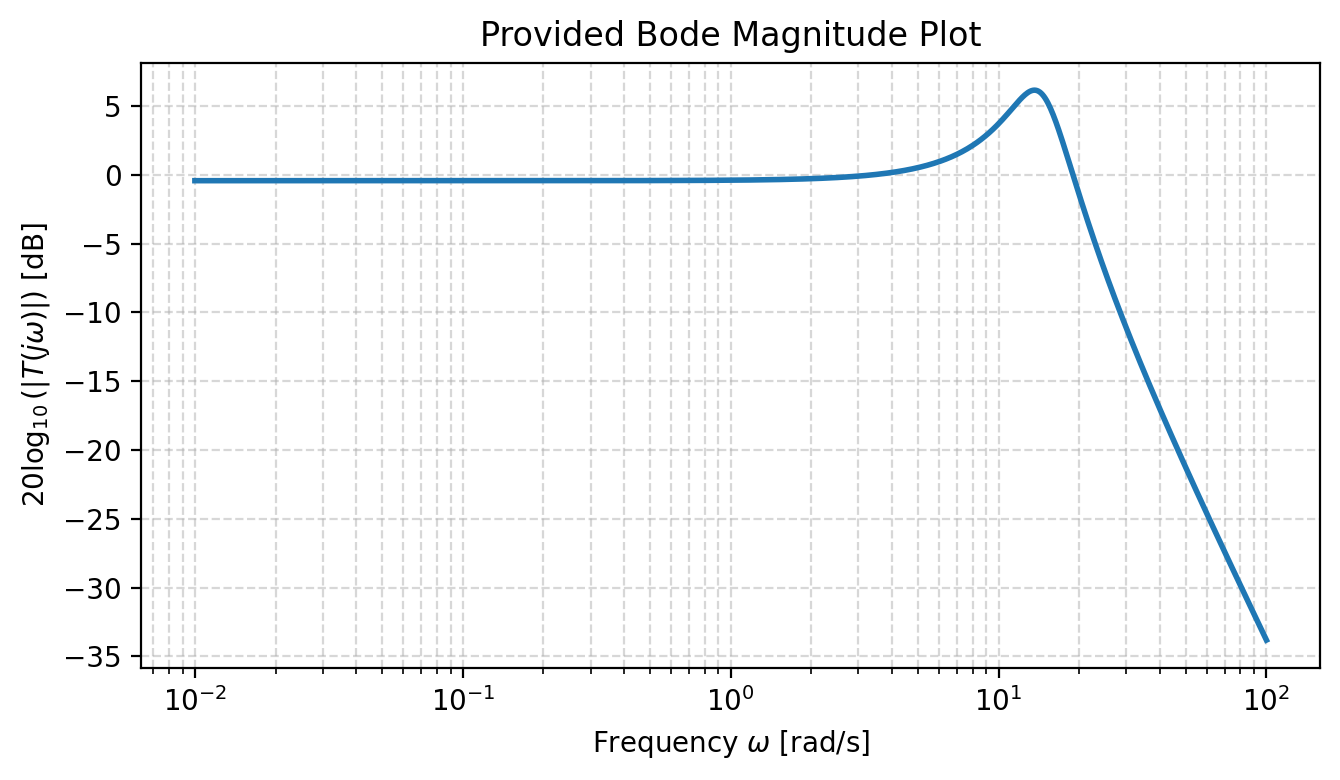
\includegraphics[width=0.92\linewidth]{bode_cltf.png}
\end{center}

\textbf{Questions}
\begin{itemize}
    \item What is the DC gain? \blankline{1.2in}
    \item Effect of controller: \blankline{2.0in}
\end{itemize}
\end{minipage}}

\end{document}